% Tao: Temporarily put the 3-in-1 screenshot here. Please move it to the proper place.
\begin{figure*}[ht]
\centering
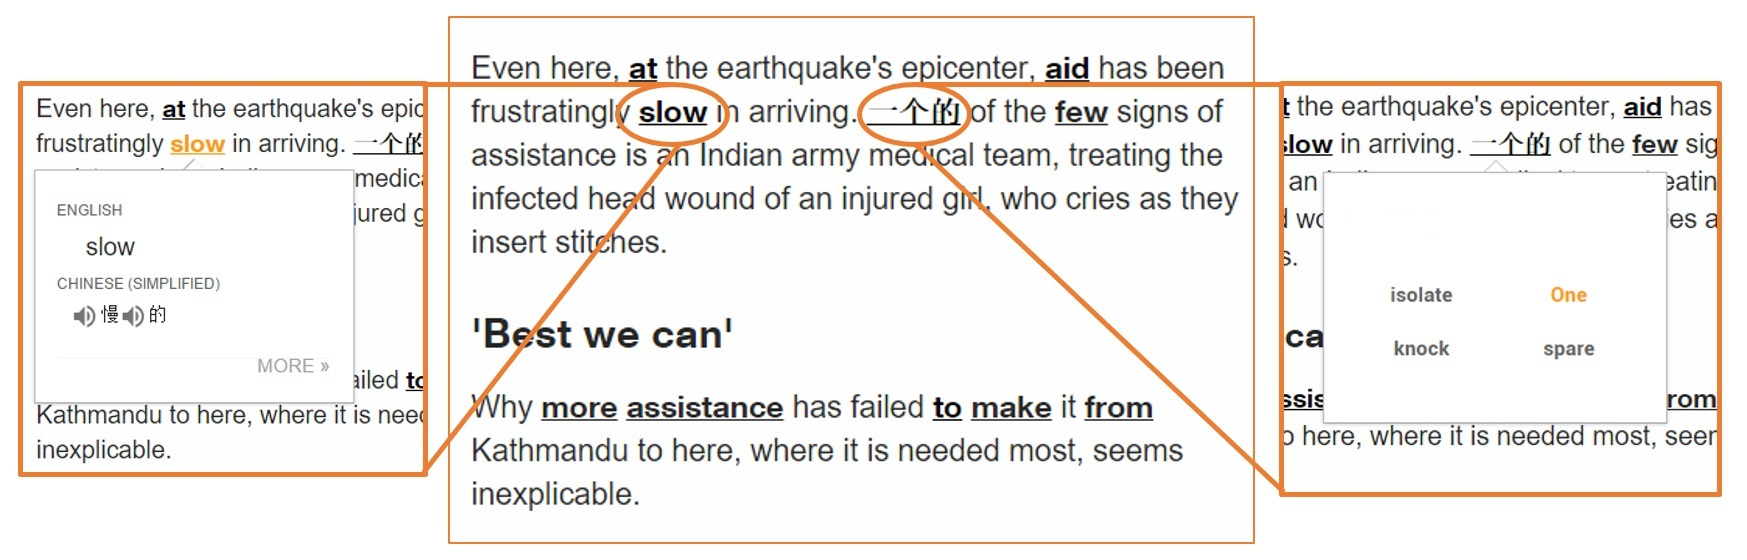
\includegraphics[width=0.99\textwidth]{chrome_extension.jpg}
\caption{Merged screenshots of our Chrome extension on the CNN English
  article {\it Treacherous journey to epicenter of deadly Nepal
    earthquake}.  Underlined components are clickable to yield
  tooltips of two different forms: (l) a definition for learning, (r)
  a multiple-choice interactive test.}
\label{fig:chrome_extension_1}
\end{figure*}

\section{The {\tt SystemA} Chrome Extension}
%%Muthu: To introduce and motivate context here
% Tao: Please mention our bilinguial dictionary 


We give a running scenario to illustrate the use of our language
learning platform, {\tt SystemA}.  When a learner browses to an
English webpage on a news website, our extension selectively replaces
certain original English words words with their Chinese translation
(Figure~\ref{fig:chrome_extension_1}, middle).  While the meaning of
the Chinese word is often apparent in context, the learner can choose
to learn more about the replaced word, by mousing over the translation
to reveal a definition tooltip (Figure~\ref{fig:chrome_extension_1},
left) to aid mastery of the Chinese word.  Once the learner has
encountered the replaced word a few times, {\tt SystemA} will assess
the learner's mastery by generating a multipl choice translation test
on the target word (Figure~\ref{fig:chrome_extension_1}, right).  Our
learning platform thus can be viewed as have three logical components:
{\it translating}, {\it learning} and {\it testing}. \\

%% \begin{figure}[ht]
%%   \centering
%%   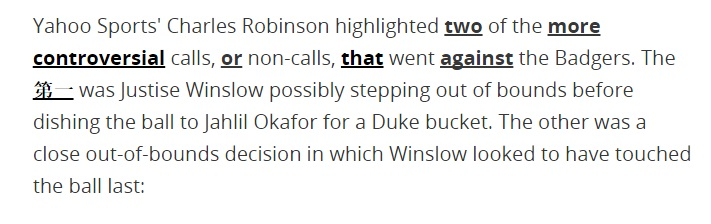
\includegraphics[width=0.45\textwidth]{software_design_2.jpg}
%%   \caption{Screen shot of Translating Component}
%%   \label{fig:software_design_2}
%% \end{figure}
{\bf Translating.}  We pass the main content of the webpage from the
extension client to our server for candidate selection and
translation.  As certain words are polysemous, the server must select
the most appropriate translation among all possible meanings.  Our
initial selection method replaces any instance of words stored in our
dictionary.  For translation, we check the word's stored meanings
against the machine translation of each sentence obtained from the
Microsoft Bing Translation API (hereafter, ``Bing'').  Matches are
deemed as correct translations and are pushed back to the Chrome
client for rendering.

%% \begin{figure}[ht]
%%   \centering
%%     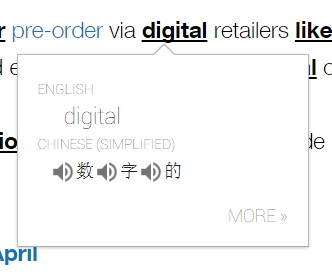
\includegraphics[width=0.3\textwidth]{software_design_4.jpg}
%%   \caption{Screen shot of popover with highlighted English word}
%%   \label{fig:software_design_4}
%% \end{figure}
%%  \begin{figure}[ht]
%%      \centering
%%     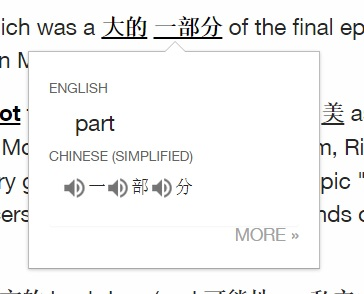
\includegraphics[width=0.3\textwidth]{software_design_5.jpg}
%%      \caption{Screen shot of popover with highlighted Chinese word}
%%      \label{fig:software_design_5}
%%  \end{figure}

{\bf Learning.} Hovering the mouse over the replacement Chinese word
causes a tooltip to appear, which gives the translation,
pronunciation, simplified and traditional written form, and a {\tt
  More} link that loads additional contextual example sentences (that
were previously translated by the backend) for the learner to study.
The more link must be clicked for activation, as we find this
two-click architecture helps to minimize latency and the loading of
unnecessary data.  The server keeps record of the learning tooltip
activations, logging the enclosing webpage URL, the target word and
the user identity.
% Min: doesn't seem to be shown, actually.  Where is an example sentence?
%  Figure \ref{fig:software_design_5} is the screen
% shot of the pop over with its example sentences.

%% \begin{figure}[ht]
%% \centering
%%   \centering
%%   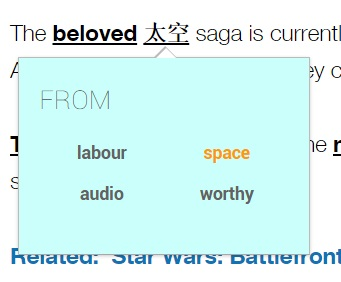
\includegraphics[width=0.3\textwidth]{software_design_7.jpg}
%%   \caption{Screenshot of English test popover}
%%   \label{fig:software_design_7}
%% \end{figure}
%% \begin{figure}[ht]
%%     \centering
%%   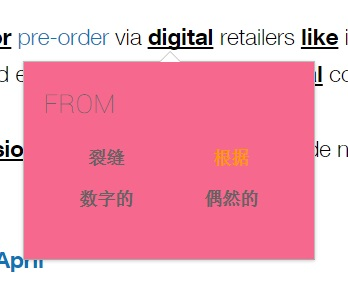
\includegraphics[width=0.3\textwidth]{software_design_8.jpg}
%%   \caption{Screen shot of Chinese test popover}
%%   \label{fig:software_design_8}
%% \end{figure}

{\bf Testing.}  After the learner encounters the same word a
pre-defined number $t=BUG$ times, {\tt SystemA} generates a MCQ test
to assess mastery.  When the learner hovers over the replaced word,
the test is shown for the learner to select the correct answer. When
an option is clicked, the server logs the selection, and the correct
answer is revealed by the client extension.  Statistics on the user's
test history are also updated.

%{\bf Classifying words category.}
% Tao: please keep the label, as I have referred it in wsd section
\subsection{News Categories}
\label{subsec:category}

A key design property of our language learning extension is only
active on certain news websites.  This is important as news articles
typically are classified with respect to a news category, such as
finance, world news, and sports.  If we know which category of news
the learner is viewing, we can leverage this knowledge for improving
the learning experience.

In particular, the category of news can impact  

domain of the 

We propose a simple way to classifying words into different categories from online news articles. To find good “category-related” words, it is essential to get the words from those already classified news articles. The following several steps described the approach we used in classifying words category information. The result of this approach is used as a possible approach in the WSD system (Section~\ref{sec:wds}) and generating suitable distractors (Section~\ref{sec:distractor}). 

{\bf Crawling news content.}
Several web crawlers are designed to get news contents from news websites. The crawler will detect URLs from each news website’s main page as and its sub-category pages. For example, there are sub-categories like “football”, “basketball” under main category “Sports”, and the crawler is able to crawl URLs from “football” page and “basketball” page as well. 

After detailed comparison of most news websites, we divided news articles into seven categories, namely “World”, “Technology”, “Sports”, “Entertainment”, “Finance”, “Health” and “Travel”. Most news articles can be classified into one of the seven categories. The web crawler will store all paragraph tags from each websites and store them as one file under one category. 

{\bf Preprocessing.}
In this step the server uses Natural Language Tool Kit \cite{edw09} for word tokenizing and POS Tagging. The server will store the POS tag of each word. After elimination of all non-English words and those words that contain special symbols, like ``O’Real", ``S\$40", all words that contains only alphabetic letters are conserved. All stop words are also eliminated as well. They are stored as lower case for the ease of future process.

{\bf Classification.}
In the classification step, the server counts the document frequency of each word in all those stored news articles, i.e. if word “scored” appeared 4 times in one article, it will only be counted as once. By following this approach we can successfully reduce the bias of some words only appear a lot of times in one article while don’t appear often in other article. As we are storing similar number of articles in each category, this approach will provide a fair comparison of each word’s popularity among different categories. After this step we will know the document frequency count of each word in different category. 
Assume C is the list of category names, and f(w, C(i))=m means word w appeared in category C(i) for m times, then the sum weight of word w as sw(w) is calculated in Equation~\ref{equation:Distractor_1}:

\begin{equation}
sw (w) = \sum_{i=1}^{n} f(w,C(i))
\label{equation:Distractor_1}
\end{equation}  

A word w is classified into category C(i) if it satisfies Equation~\ref{equation:Distractor_3}::

\begin{equation}
f (w, C(i)) - sw(w)/n >= \delta
\label{equation:Distractor_3} 
\end{equation}  

The confidence factor $\delta$ can be a positive integer between 0 and the average number of articles in each category. It means on average, the word w must appear in a specific category C(i) $\delta$ times more than it appear in other category before it can be classified into category C(i).

It is obvious that a higher confidence factor value will result in less number words getting classified, but it will result in getting words that are more accurate. A suitable confident value is selected to generating category-related words in the later section.





